\section{概要}
今回ブラックジャックの戦略を検証するためにデック数を無限に設定したものとデック数を1に設定したものの2種類の条件を用意しシミュレーションを実行した。その際に勝率、デック数、複雑性のそれぞれの観点から仮説を設定した。また、シミュレーションを実行するためのシミュレータをPython3を用いて作成した。その際にPython Software Foundation(2018)のドキュメントを参照した。以下の部分ではシミュレーションの条件設定、デック数についての説明とデック数の違いが生む影響、設定した仮説、シミュレータの詳細のそれぞれについて順に述べていく。
%今回ブラックジャックの戦略を検証するためにいくつかの仮説を立ててシミュレーションを行った。
%その際に立ててた仮説と検証の手順について以下の章で詳しく述べていく。また、検証のために
%Python3を用いてブラックジャックのシミュレータを作成したのでその詳細についても述べていく。

\bunseki{※尾崎拓海}

\section{シミュレーションの条件設定}
今回7つの戦略で実験を行う。その際、2つの条件を設定した。
\begin{itemize}
\item 条件1:デック数が無限であるとする
\item 条件2:デック数が1つであるとする
\end{itemize}
条件1は13種類のカードすべてを常に同じ確率で引くという状況に相当する。カードを何十枚、何百枚引いたとしても次に引くカードの確率は一定であり、場に出たカードに影響を受けないという状況である。\\
条件2は次に引くカードが場にあるカードに影響を受けるという状況に相当する。次に引くカードの確率は既にゲームに使用されたカードや場に出ているカードによって変動するという状況である。\\
2つの条件で比較する際に共通している条件は以下の通りである。
\begin{itemize}
\item プレイヤーの人数とディーラーの人数は一人とする。
\item ベーシックストラテジー、ベーシックストラテジー改変1、ベーシックストラテジー改変2、15以上になるまでヒットする戦略、16以上になるまでヒットする戦略、17以上になるまでヒットする戦略、18以上になるまでヒットする戦略それぞれの戦略でシミュレータを実行する。
\item ゲームの実行回数は10万回とする。
\end{itemize}
\bunseki{※尾崎拓海}

\subsection{デック数について}
今回デックはジョーカーを抜いた52枚1組を1デックと表す。例えば、8デックを使用するとした場合、1デック52枚である事から、$52×8=416$、合計416枚のカードがゲームに使用される。また、一般的にはブラックジャックで使用されるデック数は1,2,4,6,8デックのいずれかである場合が多い。\\
デック数によってデックの枚数や含まれるそれぞれのカードの枚数などが変化し、それがカードを引く確率に影響を与える。そのためブラックジャックの勝敗にも影響を及ぼす。

\bunseki{※尾崎拓海}

\subsection{デック数の違いによる影響}
今回のシミュレーションで比較するデック数無限とデック数1の双方において、10を1枚引いた後で更に続けて10を引く確率を考えてみる。
\subsubsection{デック数無限の場合}
デック数が無限である事からデックに含まれる10の枚数も同様に無限となっている。この状態のデックから10を1枚引いたとしてもデックに残っている10の枚数は変わらず無限であり、次に10を引く確率は一定となる。この事から次にデックから10を引く確率は\begin{equation}\frac{4}{52} \fallingdotseq 7.69%\end{equation}となる。\\
\subsubsection{デック数1の場合}
デック数1の場合使用するカードは52枚でありその中に10は4枚含まれている。この状態のデックから10を1枚引くとデックに含まれる10の枚数は1枚少なくなる。この事から次にデックから10を引く確率は\begin{equation}\frac{3}{51}\fallingdotseq5.88%\end{equation}となる。\\
デック数無限とデック数1の条件で10を引いた後に続けて10を引く確率を比較してみるとデック数無限のときは7.69%、デック数1の時は5.88%となり、デック数により次に引くカードの確率が変化していることが分かる。これがデック数の違いによる影響である。以下の図\ref{hogehoge}はデック数による勝率の違いを表したものである。

\begin{figure}[H]
\begin{center}

 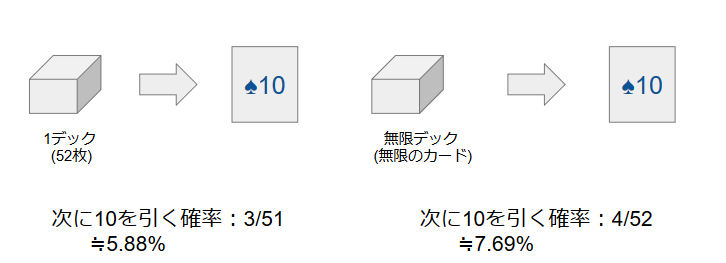
\includegraphics[width=0.7\linewidth]{./figure/DeckDiff.PNG}
 \caption{デック数による勝率の違い \label{hogehoge}}
\end{center}
\end{figure}

\bunseki{※尾崎拓海}

\section{仮説}
今回は仮説を以下のように設定した。
\begin{itemize}
\item 勝率に関して
    \begin{itemize}
        \item 仮説1.デック数が無限の時にはベーシックストラテジーの方が勝率が高い
        \item 仮説2.デック数が1の時にはベーシックストラテジー以外の勝率が高い
    \end{itemize}
\item 複雑性を考慮した場合
    \begin{itemize}
        \item 仮説3.プレイヤーの合計値が15,16,17,18以上になるまでヒットする戦略の方が性能が高い
    \end{itemize}
\item デック数を考慮した場合
    \begin{itemize}
        \item 仮説4.デック数1とデック数無限では勝率に有意な差が出る
    \end{itemize}
\end{itemize}
ベーシックストラテジーの表はデック数が無限であることを前提として導出されている。我々はこの点に着目し、デック数が有限になった際にはベーシックストラテジーよりも優れた戦略が存在するのではないか、あるいは、ベーシックストラテジーはデック数有限には対応しきれないのではないかと考えた。こうした考えから仮説1、仮説2のそれぞれを設定した。また、基準値以上になるまでヒットする戦略の方が複雑性が低くなり、性能の評価がよくなるのではないかという考えから仮説3を設定した。デック数1とデック数無限では,カードを引く確率が変化する事から、デック数が違えば勝率に有意な差が出るのではないかと考え、仮説4を設定した。
\bunseki{※尾崎拓海}

\section{検証手順}
設定した仮説を以下の手順で検証した。
\begin{enumerate}
\item ブラックジャックのシミュレータを作成
\item デック数が1の場合と無限の場合でシミュレーションを10万回実施
\item 勝った割合、負けた割合、引き分けた割合の3つを調べた
\item 得られた結果から基本戦略とその他の戦略との間の勝率に有意な差があるかどうかをカイ二乗検定を用いて調べた
\end{enumerate}
\bunseki{※尾崎拓海}

\section{ブラックジャックシミュレータ}
ベーシックストラテジーとその他の戦略を比較する事を目的に、ブラックジャックのシミュレータをプログラミング言語(Python3)を用いて作成した。このシミュレータを使用して、ベーシックストラテジー、ベーシックストラテジー改変1、ベーシックストラテジー改変2、15以上になるまでヒットする戦略、16以上になるまでヒットする戦略、17以上になるまでヒットする戦略、18以上になるまでヒットする戦略のそれぞれについて勝利回数、敗北回数、引き分けた回数の3つを調べた。ここでは、シミュレータ内部の詳細を記述していく。

\lstset{ 
   basicstyle={\ttfamily\small}, %書体の指定 
   frame=tRBl, %フレームの指定 
   framesep=10pt, %フレームと中身(コード)の間隔 
   breaklines=true, %行が長くなった場合の改行 
   linewidth=12cm, %フレームの横幅 
   lineskip=-0.5ex, %行間の調整 
   tabsize=2 %Tabを何文字幅にするかの指定 
}

\bunseki{※尾崎拓海}

\subsubsection{基本設計}
まず初めに、シミュレータの基本設計について説明する。今回作成したシミュレータではブラックジャックを行う際に必要となる要素をクラスとして表現した。具体的にはトランプのカードを
表現するカードクラスとそれを一纏めにするデッククラス、ゲーム参加者を表すクラスとそれを継承したプレイヤークラスとディーラークラス、ゲームの勝敗を判定するマネージャークラスのそれ
ぞれを定義した。これらのクラスを用いてブラックジャックのゲームを再現し、ベーシックストラテジーとその他の戦略を実行するプログラムを作成した。次に各クラスの詳細を記述していく。ソースコードは巻末の付録に全て載せてある。

\subsubsection{トランプのカードを表現するクラス}
このクラスでは実際のトランプのカードを表現するためにrankという変数にA~Kというトランプのランクを、suitという
変数にスペード、ハート、ダイヤ、クラブのスートを定義した。また、J,Q,K,Aの絵札カードは10や11と数える必要があっ
たので、ランクを数字に変換する処理もこのクラスに書き、valueという変数に入力した。%ソースコードは以下である。

\begin{comment}
\begin{itemize}
\item カードを表現するクラス
\begin{lstlisting}
class Card:
   RANKS = ('A', '2', '3', '4', '5', '6', '7', '8', '9', '10', 'J', 'Q', 'K')
   SUITS = ('Spade', 'Heart', 'Diamond', 'Club')

    # 初期化
    def __init__(self, rank, suit):
        self.rank = rank
        self.suit = suit
        self.value = int(self.getvalue())

    # ランクを数字に変換する
    def getvalue(self):
        if self.rank == 'A':
            return 11
        elif self.rank == 'J' or self.rank == 'Q' or self.rank == 'K':
            return 10
        else:
            return self.rank
\end{lstlisting}
\end{itemize}
\end{comment}

\subsubsection{デックを表現するクラス}
このクラスでは先程定義したカードクラスを利用してデックを定義した。具体的には先程のカードクラスの配列を作成
し、その中にジョーカーを除く52種類のトランプカードを作成した。このクラスの初期化時に使用するデックの数を指
定する。また、デックのシャッフルには独自に作成した関数を使用した。このシャッフル関数はPython3のrandom関数を
用いて独自に設計したものであり、引数にシャッフルを行う回数を指定する。カードの配列の長さが仮に52だった場合に
は、1~26番目のカードからランダムに取り出したカードと、27~52番目のからランダムに取り出したカードを交換する
という処理を(デック数×指定されたシャッフル回数)繰り返すという処理でシャッフル関数を作成した。%ソースコードは以下である。

\begin{comment}
\begin{itemize}
\item デックを表現するクラス
\begin{lstlisting}
class Deck:
    CARDS = [Card(rank, suit) for suit in Card.SUITS for rank in Card.RANKS]
    Cards = []
    BaseDeck = []
    for rank in Card.RANKS:
        for suit in Card.SUITS:
            # オブジェクト共有を回避するための基本となる一デッキ
            BaseDeck.append(Card(rank, suit))  

    # 初期化
    # decNum の数だけデッキを使用する
    def __init__(self, decNum):
        basedec = []
        while (decNum > 0):
            basedec += self.BaseDeck
            decNum -= 1
        self.Cards = basedec
        self.current = 0

    # シャッフルをする関数
    # 引数に入れる数字によりシャッフルの回数を制御
    def shuffle(self, shuffleNum):
        self.current = 0
        while shuffleNum > 0:
            cut1 = random.randrange(0, len(self.Cards) / 2)
            cut2 = random.randrange(len(self.Cards) / 2, len(self.Cards))
            temp = self.Cards[cut1]
            self.Cards[cut1] = self.Cards[cut2]
            self.Cards[cut2] = temp
            shuffleNum -= 1
\end{lstlisting}
\end{itemize}
\end{comment}

\subsubsection{ゲーム参加者を表すスーパークラス}
このクラスでは自身の手札とその手札の合計値、手札に含まれるAの枚数、バーストしているかどうかのフラグ、手札
がブラックジャックとなっているかどうかのフラグのそれぞれを定義している。手札に含まれるAの枚数は自身の手札
の合計値を計算する時と、ブラックジャックの条件を満たしているかどうかを判別する際に使用した。また手札の合計
値を返す関数を定義し、その内側で自身がバーストしているかどうかの判定も行っている。%ソースコードは以下である。

\begin{comment}
\begin{itemize}
\item ゲーム参加者を表すスーパークラス
\begin{lstlisting}
class GamePlayer:

    # 初期化関数
    def __init__(self):
        # 参加者の手札
        self.cards = []  
        # 参加者の手札の合計値
        self.total = 0  
        # 参加者の手札に含まれるAの枚数
        self.acetotal = 0  
        # 1として数えたAの枚数
        self.usedace = 0  
        # バーストしているかどうか
        self.burst = False  
        # ナチュラルブラックジャックを満たしているかどうか
        self.naturalbj = False 
        # 手札の合計値が21 になっているかどうか
        self.normalbj = False  

    # 子オブジェクトから呼び出せる初期化関数
    def initialize(self):
        self.cards = []
        self.total = 0
        self.acetotal = 0
        self.usedace = 0
        self.burst = False
        self.naturalbj = False
        self.normalbj = False

    # ゲームプレイヤーの手札の合計値を返す関数
    def totalvalue(self):
        i = 0
        self.total = 0
        self.acetotal = 0
        cardnum = len(self.cards)

        while i < cardnum:
            if (self.cards[i].rank == 'A'):
                self.acetotal += 1
            self.total += self.cards[i].value
            i += 1
        self.total -= 10 * self.usedace

        # プレイヤーのバースト判定の処理
        if (self.total > 21):
            if (self.acetotal - self.usedace > 0):
                self.total -= 10
                self.usedace += 1
                if (self.total > 21):
                    self.burst = True
            else:
                self.burst = True

\end{lstlisting}
\end{itemize}
\end{comment}

\subsubsection{プレイヤークラス}
このクラスは先のゲーム参加者を表すスーパークラスを継承しており、ゲームに参加しているプレイヤーを表現して
いる。プレイヤークラスでは新たに自身の名前を表す変数と自身の勝利回数、敗北回数を記録する変数を定義した。
またこのクラスでは新しく、カードを受け取る関数とヒットを行う関数、スタンドを行う関数、勝利回数と敗北回数
を増加させる関数を作成した。%ソースコードは以下である。

\begin{comment}
\begin{itemize}
\item プレイヤークラス
\begin{lstlisting}
class Player(GamePlayer):
    # プレイヤーの初期化
    def __init__(self, name):
        self.name = name  # プレイヤーの名前
        self.totalwin = 0  # プレイヤーの勝利回数
        self.totallose = 0  # プレイヤーの敗北回数
        super().__init__()

    # プレイヤーがカードを受け取る時に使用する関数
    def dealedcard(self, card):
        self.cards.append(card)

    # プレイヤー側のヒットの処理
    def hit(self, dealer):
        self.dealedcard(dealer.dealcard())
        self.showhands()

    # プレイヤー側のスタンドの処理
    def stand(self):
        pass

    # プレイヤーの勝利回数を増やす
    def addtotalwin(self):
        self.totalwin += 1

    # プレイヤーの敗北回数を増やす
    def addtotallose(self):
        self.totallose += 1

\end{lstlisting}
\end{itemize}
\end{comment}

\subsubsection{ディーラークラス}
このクラスは先のゲーム参加者を表すスーパークラスを継承しており、ゲームのディーラーを表現しているクラス
となっている。ディーラークラスの中でデックをインスタンス化してディーラー側がデックを所持している事を表
現している。このクラスでは新しく、デックのシャッフル回数という変数を定義した。また、このクラスではカード
を配る関数、ディーラーの手札合計が17を超えるまでカードを引き続ける関数を作成した。カードを配る関数についてはデック数有限の時とデック数無限の時とで処理を変更している。%ソースコードは以下である。

\begin{comment}
\begin{itemize}
\item ディーラークラス(デック数有限)
\begin{lstlisting}
class Dealer(GamePlayer):
    # ディーラーの初期化
    def __init__(self, deckNum):
        self.deck = Deck(deckNum)
        # ディーラーがシャッフルする回数。今回は一万回シャッフルする。
        self.shufflenum = 10000
        self.deck.shuffle(deckNum * self.shufflenum)
        super().__init__()

    # カードを配る関数
    def dealcard(self):
        ''' デック数有限の際はこちらのコメントアウトを解除する '''
        card = self.deck.Cards[self.deck.current]
        self.deck.current += 1
        
        ''' デック数無限の際にはこちらのコメントアウトを解除する '''
        # randomcard = random.randrange(13);
        # card = Card(Card.RANKS[randomcard], Card.SUITS[0])
        # return card

    # 一番最初にカードを配る際の関数
    def firstdeal(self, player):
        super().__init__()
        for x in player:
            x.initialize()
        firstdeal = 2
        while firstdeal > 0:
            self.cards.append(self.dealcard())
            for x in player:
                x.cards.append(self.dealcard())
            firstdeal -= 1

    # 合計が17 を超えるまで引き続ける処理
    def continuehit(self):
        self.totalvalue()
        while (self.total < 17):
            self.cards.append(self.dealcard())
            self.totalvalue()

\end{lstlisting}
\end{itemize}
\end{comment}

\subsubsection{ゲームマネージャークラス}
このクラスは主にゲームの勝敗判定に使用している。プレイヤーとディーラーの手札の合計値を比較し勝敗を判定
する関数と、手札がブラックジャックになっているかどうかを判定する関数を作成した。勝敗判定のタイミングで
プレイヤーの勝利回数、敗北回数のそれぞれを記録している。%ソースコードは以下である。

\begin{comment}
\begin{itemize}
\item ゲームマネージャークラス
\begin{lstlisting}
class GameManager:
    def __init__(self, players, dealer):
        self.players = players
        self.dealer = dealer
        self.checkdeal = True

    # 各プレイヤーとディーラーとの間で勝敗を決める
    def judge(self):
        for x in self.players:
            self.checkblackjack(x)
        self.checkblackjack(self.dealer)
        for player in self.players:
            if player.burst == True:
                player.addtotallose()
            elif player.burst == False and self.dealer.burst == True:
                player.addtotalwin()
            elif player.total > self.dealer.total:
                player.addtotalwin()
            elif player.total < self.dealer.total:
                player.addtotallose()
            elif player.total == self.dealer.total:
                if player.naturalbj and self.dealer.naturalbj:
                elif player.naturalbj and self.dealer.normalbj:
                    player.addtotalwin()
                elif player.normalbj and self.dealer.naturalbj:
                    player.addtotallose()
                elif player.normalbj and self.dealer.normalbj:
                    pass
                else:
                    pass
\end{lstlisting}
\end{itemize}
\end{comment}

\subsubsection{メイン関数}
以上のクラスを用いてメイン関数にブラックジャックのゲームを記述した。以下にプログラムの実行手順を示す。
\begin{enumerate}
    \item ゲームに参加するプレイヤーを作成。今回はプレイヤーを一人のみ作成した。
    \item ディーラーを作成。
    \item カットカードを定義。カットカードを挟む位置はデックの半分の位置とした。
    \item ゲーム全体の実行回数を定義。今回は10万回とした。
    \item プレイヤーの戦略を配列形式で定義した。
    \item ゲームを繰り返すwhile文を作成し、ループ回数を10万回とした。
    \begin{enumerate}
        \item デックからカットカードが出てきたかを確認する。もし出てきていればデックをシャッフルする。
	  \item ディーラーが自身を含む各プレイヤーに初期カードを配る。
	  \item プレイヤーは自身の戦略に沿った行動を選択する。
	  \item すべてのプレイヤーの行動が終了したことを確認後にディーラーが行動を開始する
	  \item ディーラーの行動終了後に、勝敗判定を行う。
    \end{enumerate}
\end{enumerate}

\subsubsection{未実装の機能について}
今回のシミュレーションでは条件を簡単にするためにヒットとスタンドの処理のみを使用しており、ダブルダウン、スプリット、サレンダー、インシュランス、イーブンマネーについては実装していない。ブラックジャックのすべてのルールをプログラム上に再現できているわけではな
いので、後期の活動でダブルダウン、スプリット、サレンダー、インシュランス、イーブンマネーを追加した完全版のシミュレータを作成する。
\bunseki{※尾崎拓海}
